\section{Ejercicios}

\subsection{Ejercicios de construcción - Pappus}

\begin{section-exercise}
    Aplicar el teorema de Pappus, dada la disposición \hspace{0.3cm}
    \begin{tabular}{|c|c|c|}
        \hline
        A&B&C \\\hline
        F&D&E \\\hline\hline
        && \\\hline
    \end{tabular}
    \vspace*{\fill}
    \begin{figure}[H]
        \centering
        
%dash pattern=on 5pt off 2pt
%[fill = white, rounded corners = 5pt, inner sep=0.8pt]
\begin{tikzpicture}[scale = 1.2]
    \clip(-7.18,-0.99) rectangle (4.94,8.68);
    \draw [line width=1.2pt] (-3.5,4.81) circle (2.98cm);
    \begin{scriptsize}
        \normalsize
        \fill [color=black] (-4.5,7.62) circle (2.5pt);
        \draw[color=black] (-4.75,7.97) node {$A$};
        \fill [color=black] (-2.24,2.11) circle (2.5pt);
        \draw[color=black] (-1.96,1.72) node {$B$};
        \fill [color=black] (-5.84,2.97) circle (2.5pt);
        \draw[color=black] (-6.26,2.86) node {$C$};
        \fill [color=black] (-0.91,3.34) circle (2.5pt);
        \draw[color=black] (-0.54,3.22) node {$D$};
        \fill [color=black] (-0.52,4.85) circle (2.5pt);
        \draw[color=black] (-0.13,5.03) node {$E$};
        \fill [color=black] (-0.72,5.86) circle (2.5pt);
        \draw[color=black] (-0.4,6.13) node {$F$};
    \end{scriptsize}
\end{tikzpicture}
    \end{figure}
    \vspace*{\fill}
\end{section-exercise}

\newpage
\begin{section-exercise}
    Aplicar el teorema de Pappus, dada la disposición \hspace{0.3cm}
    \begin{tabular}{|c|c|c|}
        \hline
        E&D&F \\\hline
        A&C&B \\\hline\hline
        && \\\hline
    \end{tabular}
    \vspace*{\fill}
    \begin{figure}[H]
        \centering
        
%dash pattern=on 5pt off 2pt
%[fill = white, rounded corners = 4pt, inner sep = 1pt]
\begin{tikzpicture}[scale = 1.5]
    \clip(-5.28,-5.51) rectangle (3.8,8.27);
    \draw [line width=1.2pt,domain=-5.28:3.8] plot(\x,{(--8.31-7.4*\x)/-1.15});
    \draw [line width=1.2pt,domain=-5.28:3.8] plot(\x,{(--11.9--3.51*\x)/-0.31});
    \begin{scriptsize}
        \normalsize
        \fill [color=black] (1.98,5.57) circle (2.5pt);
        \draw[color=black] (2.49,5.81) node {$A$};
        \fill [color=black] (0.84,-1.83) circle (2.5pt);
        \draw[color=black] (1.39,-1.79) node {$B$};
        \fill [color=black] (1.42,1.91) circle (2.5pt);
        \draw[color=black] (1.89,1.99) node {$C$};
        \fill [color=black] (-3.6,2.44) circle (2.5pt);
        \draw[color=black] (-4.06,2.39) node {$D$};
        \fill [color=black] (-3.92,5.95) circle (2.5pt);
        \draw[color=black] (-4.39,5.74) node {$E$};
        \fill [color=black] (-3.09,-3.36) circle (2.5pt);
        \draw[color=black] (-3.6,-3.67) node {$F$};
    \end{scriptsize}
\end{tikzpicture}
    \end{figure}
    \vspace*{\fill}
\end{section-exercise}

\newpage
\begin{section-exercise}
    Aplicar el teorema de Pappus, dada la disposición \hspace{0.3cm}
    \begin{tabular}{|c|c|c|}
        \hline
        B&A&C \\\hline
        F&E&D \\\hline\hline
        && \\\hline
    \end{tabular}
    \vspace*{\fill}
    \begin{figure}[H]
        \centering
        
%dash pattern=on 5pt off 2pt
%[fill = white, rounded corners = 4pt, inner sep = 1pt]
\begin{tikzpicture}[scale = 1.5]
    \clip(-5.25,-4.58) rectangle (5.59,8.27);
    \draw [line width=1.2pt,domain=-5.25:5.59] plot(\x,{(-9.3--0.81*\x)/-1.31});
    \draw [line width=1.2pt,domain=-5.25:5.59] plot(\x,{(--1.79--2.7*\x)/-0.74});
    \begin{scriptsize}
        \normalsize
        \fill [color=black] (3.68,4.81) circle (2.5pt);
        \draw[color=black] (4.18,5.05) node {$A$};
        \fill [color=black] (2.37,5.62) circle (2.5pt);
        \draw[color=black] (2.92,5.67) node {$B$};
        \fill [color=black] (0.42,6.83) circle (2.5pt);
        \draw[color=black] (0.89,6.89) node {$C$};
        \fill [color=black] (-0.74,0.27) circle (2.5pt);
        \draw[color=black] (-1.19,0.22) node {$D$};
        \fill [color=black] (-1.48,2.97) circle (2.5pt);
        \draw[color=black] (-1.96,2.75) node {$E$};
        \fill [color=black] (0.14,-2.93) circle (2.5pt);
        \draw[color=black] (-0.36,-3.24) node {$F$};
    \end{scriptsize}
\end{tikzpicture}
    \end{figure}
    \vspace*{\fill}
\end{section-exercise}

\newpage
\begin{section-exercise}
    Aplicar el teorema de Pappus, dada la disposición \hspace{0.3cm}
    \begin{tabular}{|c|c|c|}
        \hline
        A&C&B \\\hline
        F&D&E \\\hline\hline
        && \\\hline
    \end{tabular}
    \vspace*{\fill}
    \begin{figure}[H]
        \centering
        
%dash pattern=on 5pt off 2pt
%[fill = white, rounded corners = 4pt, inner sep = 1pt]
\begin{tikzpicture}[scale = 1.3]
    \clip(-5.21,-5.51) rectangle (7.65,8.22);
    \draw [line width=1.2pt,domain=-5.21:7.65] plot(\x,{(-22.09--7.33*\x)/-3.87});
    \draw [line width=1.2pt,domain=-5.21:7.65] plot(\x,{(-6.87-2.56*\x)/0.48});
    \begin{scriptsize}
        \normalsize
        \fill [color=black] (3.06,-0.09) circle (3pt);
        \draw[color=black] (3.51,0.22) node {$A$};
        \fill [color=black] (-0.81,7.24) circle (3pt);
        \draw[color=black] (-0.55,7.77) node {$B$};
        \fill [color=black] (4.86,-3.5) circle (3pt);
        \draw[color=black] (5.19,-3.2) node {$C$};
        \fill [color=black] (-3.6,4.9) circle (3pt);
        \draw[color=black] (-4.06,4.85) node {$D$};
        \fill [color=black] (-3.13,2.35) circle (3pt);
        \draw[color=black] (-3.6,2.13) node {$E$};
        \fill [color=black] (-1.79,-4.79) circle (3pt);
        \draw[color=black] (-2.29,-5.11) node {$F$};
    \end{scriptsize}
\end{tikzpicture}
    \end{figure}
    \vspace*{\fill}
\end{section-exercise}

\newpage
\begin{section-exercise}
    Aplicar el teorema de Pappus, dada la disposición \hspace{0.3cm}
    \begin{tabular}{|c|c|c|}
        \hline
        B&F&E \\\hline
        A&C&D \\\hline\hline
        && \\\hline
    \end{tabular}
    \vspace*{\fill}
    \begin{figure}[H]
        \centering
        
%dash pattern=on 5pt off 2pt
%[fill = white, rounded corners = 4pt, inner sep = 1pt]
\begin{tikzpicture}[scale = 1]
    \clip(-4.56,-5.46) rectangle (12.59,8.27);
    \draw [line width=1.2pt,domain=-4.56:12.59] plot(\x,{(--37.46--1.84*\x)/-12.37});
    \draw [line width=1.2pt,domain=-4.56:12.59] plot(\x,{(-3.3-0.5*\x)/-3.11});
    \begin{scriptsize}
        \normalsize
        \fill [color=black] (8.2,-4.25) circle (4pt);
        \draw[color=black] (8.15,-3.62) node {$F$};
        \fill [color=black] (-4.18,-2.41) circle (4pt);
        \draw[color=black] (-4.2,-1.83) node {$B$};
        \fill [color=black] (-0.81,-2.91) circle (4pt);
        \draw[color=black] (-0.86,-2.29) node {$E$};
        \fill [color=black] (1.89,1.37) circle (4pt);
        \draw[color=black] (1.77,1.85) node {$D$};
        \fill [color=black] (-1.22,0.87) circle (4pt);
        \draw[color=black] (-1.36,1.42) node {$C$};
        \fill [color=black] (4.96,1.86) circle (4pt);
        \draw[color=black] (4.85,2.39) node {$A$};
    \end{scriptsize}
\end{tikzpicture}
    \end{figure}
    \vspace*{\fill}
\end{section-exercise}




\newpage
\subsection{Ejercicios de perspectiva - Desargues}

\begin{section-exercise}
    Encuentre, con la ayuda de una regla, el punto y la recta para los cuales los triángulos \theTriangle{ABC} y \theTriangle{XYZ} están en perspectiva.
    \vspace*{\fill}
    \begin{figure}[H]
        \centering
        \definecolor{ttqqcc}{rgb}{0.33,0.33,0.33}
%dash pattern=on 5pt off 2pt
%[fill = white, rounded corners = 4pt, inner sep = 1pt]
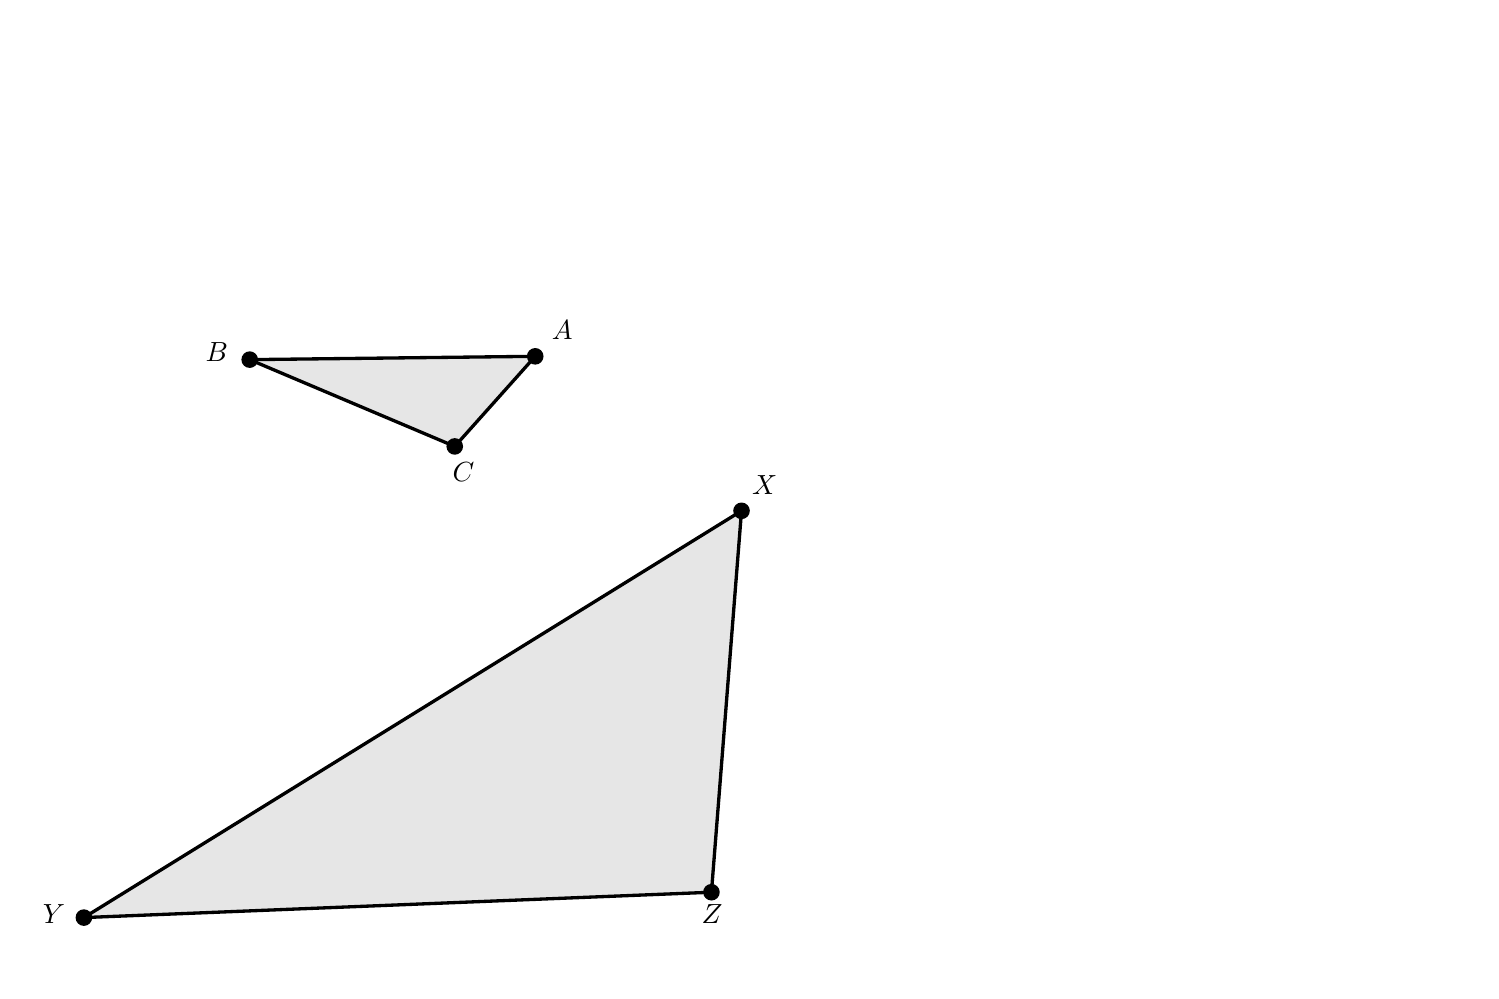
\begin{tikzpicture}[scale = 0.2]
    \clip(-25.62,-26.27) rectangle (66,33.59);
    \fill[line width=0pt,color=ttqqcc,fill=ttqqcc,fill opacity=0.15] (6.61,12.72) -- (-11.52,12.51) -- (1.5,7) -- cycle;
    \fill[line width=0pt,color=ttqqcc,fill=ttqqcc,fill opacity=0.15] (19.71,2.91) -- (-22.05,-22.92) -- (17.8,-21.31) -- cycle;
    \draw [line width=1.2pt] (6.61,12.72)-- (-11.52,12.51);
    \draw [line width=1.2pt] (-11.52,12.51)-- (1.5,7);
    \draw [line width=1.2pt] (1.5,7)-- (6.61,12.72);
    \draw [line width=1.2pt] (19.71,2.91)-- (-22.05,-22.92);
    \draw [line width=1.2pt] (-22.05,-22.92)-- (17.8,-21.31);
    \draw [line width=1.2pt] (17.8,-21.31)-- (19.71,2.91);
    \begin{scriptsize}
        \normalsize
        \fill [color=black] (-11.52,12.51) circle (15pt);
        \draw[color=black] (-13.61,13.01) node {$B$};
        \fill [color=black] (1.5,7) circle (15pt);
        \draw[color=black] (2.06,5.38) node {$C$};
        \fill [color=black] (6.61,12.72) circle (15pt);
        \draw[color=black] (8.33,14.37) node {$A$};
        \fill [color=black] (19.71,2.91) circle (15pt);
        \draw[color=black] (21.18,4.55) node {$X$};
        \fill [color=black] (-22.05,-22.92) circle (15pt);
        \draw[color=black] (-23.95,-22.72) node {$Y$};
        \fill [color=black] (17.8,-21.31) circle (15pt);
        \draw[color=black] (17.84,-22.72) node {$Z$};
    \end{scriptsize}
\end{tikzpicture}
    \end{figure}
    \vspace*{\fill}
\end{section-exercise}

\newpage
\begin{section-exercise}
    Encuentre, con la ayuda de una regla, el punto y la recta para los cuales los triángulos \theTriangle{ABC} y \theTriangle{XYZ} están en perspectiva.
    \vspace*{\fill}
    \begin{figure}[H]
        \centering
        
%dash pattern=on 5pt off 2pt
%[fill = white, rounded corners = 5pt, inner sep=0.8pt]
\begin{tikzpicture}[scale = 0.95]
    \clip(-12.74,-2.62) rectangle (4.52,7.28);
    \draw [line width=1.2pt] (0.35,1.15) circle (2.64cm);
    \begin{scriptsize}
        \normalsize
        \fill [color=black] (-1.56,3.64) circle (3pt);
        \fill[color=black]  (3.62,4.09) circle (3pt);
        \fill[color=black] (2.68,-0.65) circle (3pt);
        \fill [color=black] (-0.26,-2.07) circle (3pt);
        \fill [color=black] (1.42,3.9) circle (3pt);
        \fill [color=black] (-2.67,0.54) circle (3pt);

        \draw[color=black] (-1.79,4.09) node {$A$};
        \draw[color=black] (3.84,4.47) node {$D$};
        \draw[color=black] (3.1,-0.63) node {$F$};
        \draw[color=black] (0.1,-2.23) node {$B$};
        \draw[color=black] (1.34,4.33) node {$E$};
        \draw[color=black] (-3.03,0.23) node {$C$};
    \end{scriptsize}
\end{tikzpicture}
    \end{figure}
    \vspace*{\fill}
\end{section-exercise}

\newpage
\begin{section-exercise}
    Encuentre, con la ayuda de una regla, el punto y la recta para los cuales los triángulos \theTriangle{SET} y \theTriangle{DHR} están en perspectiva.
    \vspace*{\fill}
    \begin{figure}[H]
        \centering
        \definecolor{ttqqcc}{rgb}{0.33,0.33,0.33}
%dash pattern=on 5pt off 2pt
%[fill = white, rounded corners = 4pt, inner sep = 1pt]
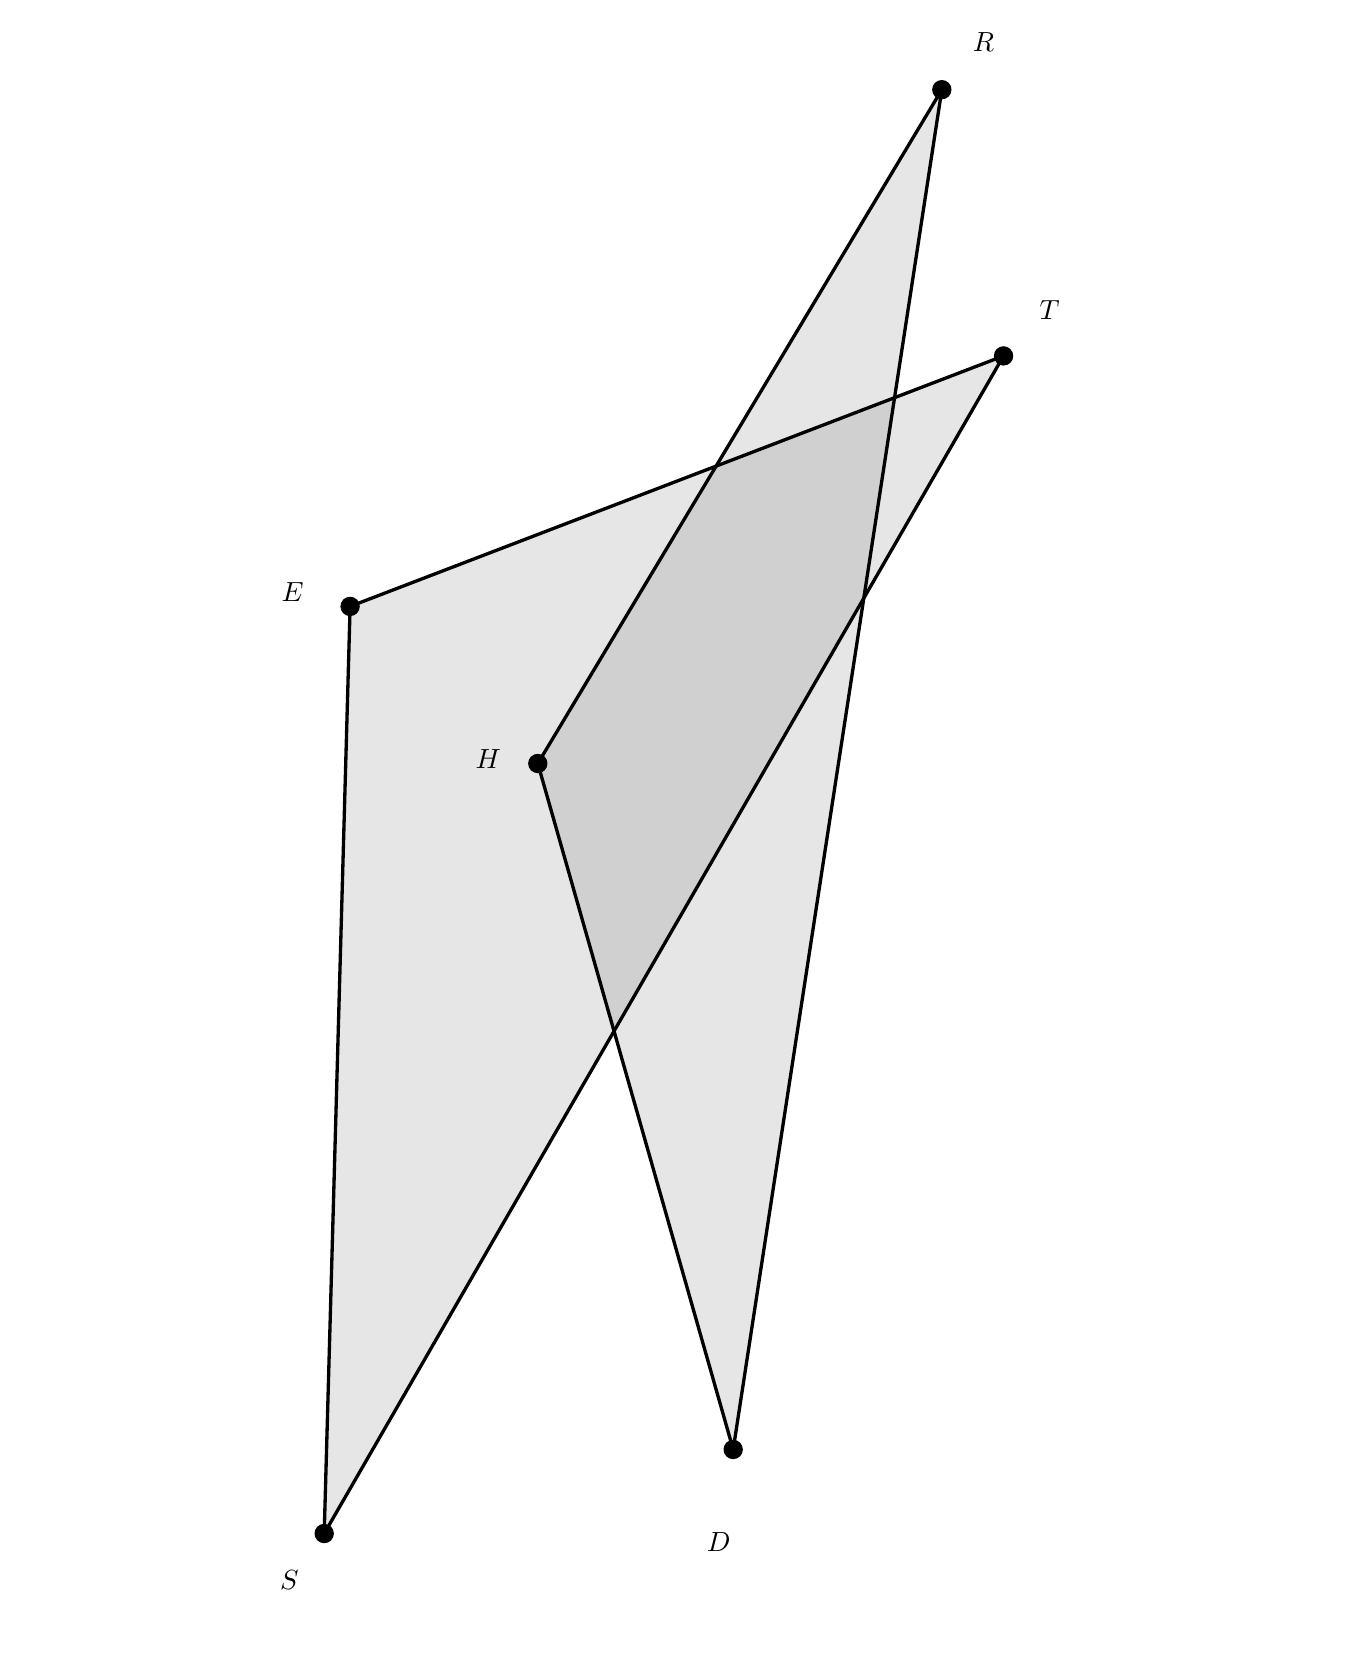
\begin{tikzpicture}[scale = 0.35]
    \clip(-25.62,-26.69) rectangle (21.49,31.61);
    \fill[line width=0pt,color=ttqqcc,fill=ttqqcc,fill opacity=0.15] (9.79,19.7) -- (-13.92,10.61) -- (-14.86,-23.03) -- cycle;
    \fill[line width=0pt,color=ttqqcc,fill=ttqqcc,fill opacity=0.15] (7.55,29.36) -- (-7.11,4.91) -- (-0.02,-19.98) -- cycle;
    \draw [line width=1.2pt] (9.79,19.7)-- (-13.92,10.61);
    \draw [line width=1.2pt] (-13.92,10.61)-- (-14.86,-23.03);
    \draw [line width=1.2pt] (-14.86,-23.03)-- (9.79,19.7);
    \draw [line width=1.2pt] (7.55,29.36)-- (-7.11,4.91);
    \draw [line width=1.2pt] (-7.11,4.91)-- (-0.02,-19.98);
    \draw [line width=1.2pt] (-0.02,-19.98)-- (7.55,29.36);
    \begin{scriptsize}
        \normalsize
        \fill [color=black] (-13.92,10.61) circle (10pt);
        \draw[color=black] (-16.01,11.13) node {$E$};
        \fill [color=black] (-14.86,-23.03) circle (10pt);
        \draw[color=black] (-16.12,-24.7) node {$S$};
        \fill [color=black] (9.79,19.7) circle (10pt);
        \draw[color=black] (11.46,21.37) node {$T$};
        \fill [color=black] (7.55,29.36) circle (10pt);
        \draw[color=black] (9.06,31.08) node {$R$};
        \fill [color=black] (-7.11,4.91) circle (10pt);
        \draw[color=black] (-8.91,5.07) node {$H$};
        \fill [color=black] (-0.02,-19.98) circle (10pt);
        \draw[color=black] (-0.55,-23.35) node {$D$};
    \end{scriptsize}
\end{tikzpicture}
    \end{figure}
    \vspace*{\fill}
\end{section-exercise}

\newpage
\begin{section-exercise}
    Encuentre, con la ayuda de una regla, el punto y la recta para los cuales los triángulos \theTriangle{DEF} y \theTriangle{ABC} están en perspectiva.
    \vspace*{\fill}
    \begin{figure}[H]
        \centering
        
%dash pattern=on 5pt off 2pt
%[fill = white, rounded corners = 5pt, inner sep=0.8pt]
\begin{tikzpicture}[scale = 1.5]
    \clip(-5.52,-3.47) rectangle (4.73,6.98);
    \draw [line width=1.2pt] (0.35,1.15) circle (2.64cm);
    \begin{scriptsize}
        \normalsize
        \fill [color=black] (2.03,3.19) circle (2.0pt);
        \fill [color=black] (-1.51,6.12) circle (2.0pt);
        \draw[color=black] (-1.64,6.61) node {$A$};
        \fill [color=black] (-2.58,-0.44) circle (2.0pt);
        \draw[color=black] (-2.89,-0.64) node {$B$};
        \fill [color=black] (0.95,-1.99) circle (2.0pt);
        \draw[color=black] (1.38,-2.16) node {$C$};
        \fill [color=black] (3.08,0.16) circle (2.0pt);
        \draw[color=black] (3.45,-0.07) node {$D$};
        \fill [color=black] (2.89,2.5) circle (2.0pt);
        \draw[color=black] (3.08,2.88) node {$E$};
        \fill [color=black] (2.02,3.2) circle (2.0pt);
        \draw[color=black] (2.2,3.56) node {$F$};
    \end{scriptsize}
\end{tikzpicture}
    \end{figure}
    \vspace*{\fill}
\end{section-exercise}

\newpage
\begin{section-exercise}
    Encuentre, con la ayuda de una regla, el punto y la recta para los cuales los triángulos \theTriangle{FED} y \theTriangle{XYZ} están en perspectiva.
    \vspace*{\fill}
    \begin{figure}[H]
        \centering
        \definecolor{ttqqff}{rgb}{0.33,0.33,0.33}
%dash pattern=on 5pt off 2pt
%[fill = white, rounded corners = 4pt, inner sep = 1pt]
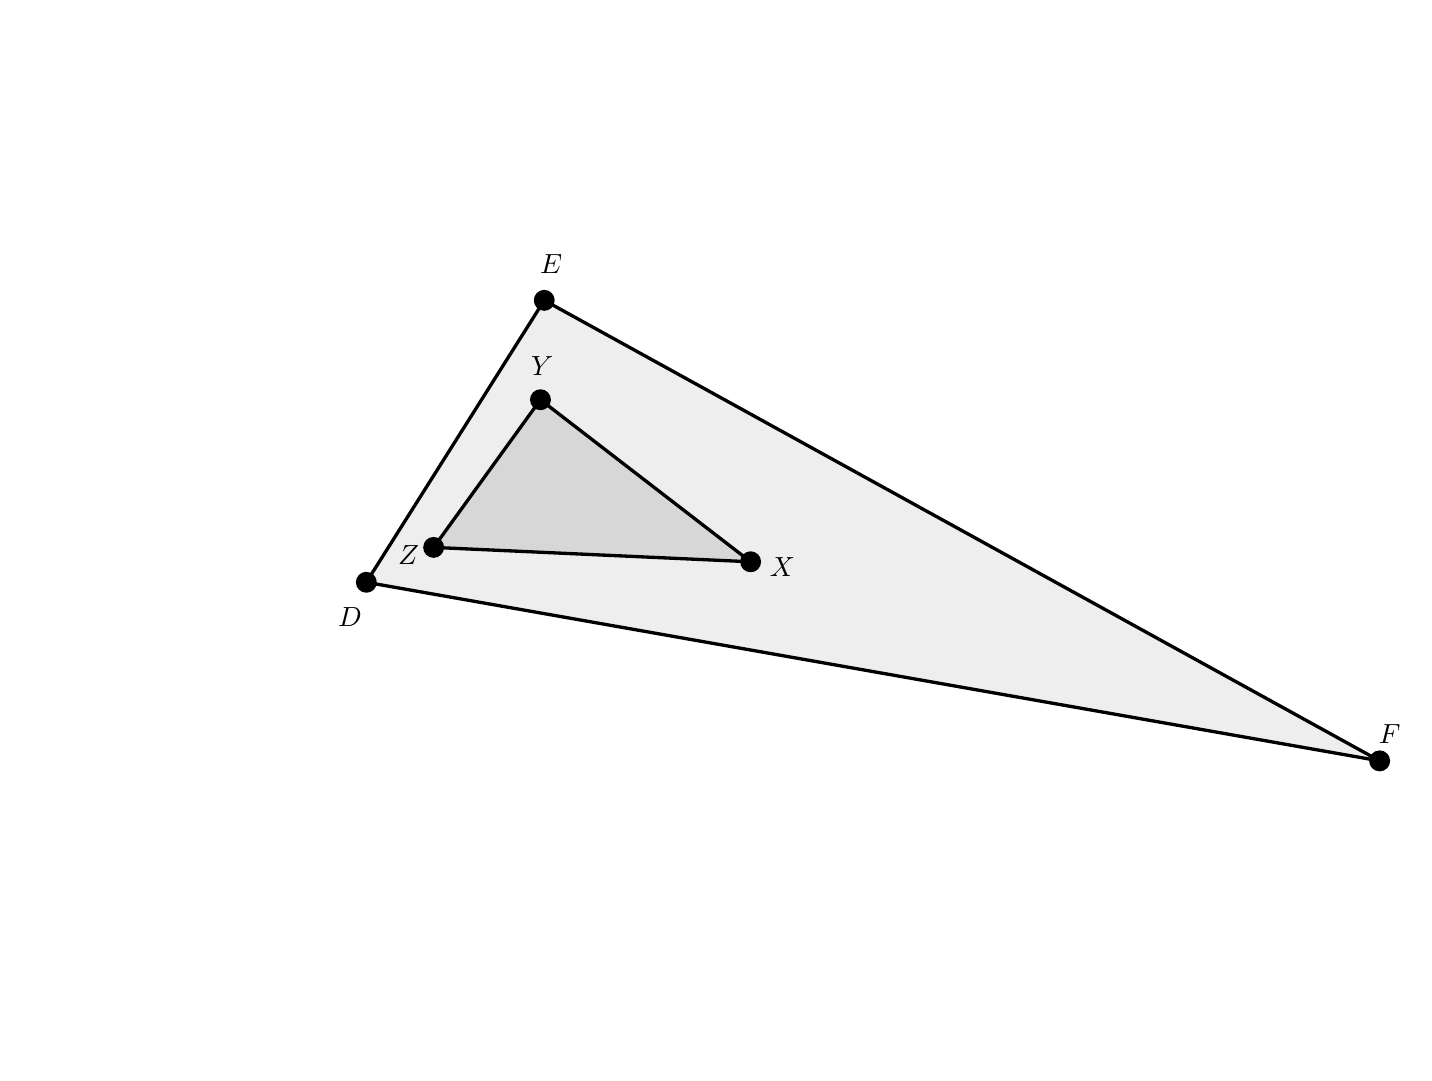
\begin{tikzpicture}[scale = 0.21]
    \clip(-29.39,-11.38) rectangle (53.84,50.63);
    \fill[line width=0pt,color=ttqqff,fill=ttqqff,fill opacity=0.15] (14.33,18.33) -- (1.62,28.13) -- (-4.84,19.2) -- cycle;
    \fill[line width=0pt,color=ttqqff,fill=ttqqff,fill opacity=0.1] (-8.91,17.09) -- (1.85,34.14) -- (52.37,6.29) -- cycle;
    \draw [line width=1.2pt] (14.33,18.33)-- (1.62,28.13);
    \draw [line width=1.2pt] (1.62,28.13)-- (-4.84,19.2);
    \draw [line width=1.2pt] (-4.84,19.2)-- (14.33,18.33);
    \draw [line width=1.2pt] (-8.91,17.09)-- (1.85,34.14);
    \draw [line width=1.2pt] (1.85,34.14)-- (52.37,6.29);
    \draw [line width=1.2pt] (52.37,6.29)-- (-8.91,17.09);
    \begin{scriptsize}
        \normalsize
        \fill [color=black] (1.62,28.13) circle (18pt);
        \draw[color=black] (1.73,30.18) node {$Y$};
        \fill [color=black] (-4.84,19.2) circle (18pt);
        \draw[color=black] (-6.35,18.76) node {$Z$};
        \fill [color=black] (14.33,18.33) circle (18pt);
        \draw[color=black] (16.26,18.01) node {$X$};
        \fill [color=black] (-8.91,17.09) circle (18pt);
        \draw[color=black] (-9.9,15) node {$D$};
        \fill [color=black] (1.85,34.14) circle (18pt);
        \draw[color=black] (2.27,36.31) node {$E$};
        \fill [color=black] (52.37,6.29) circle (18pt);
        \draw[color=black] (52.98,7.89) node {$F$};
    \end{scriptsize}
\end{tikzpicture}
    \end{figure}
    \vspace*{\fill}
\end{section-exercise}